
\documentclass[a4paper,10pt]{article}
\usepackage[top=2cm, left=2.5cm, right=2.5cm, bottom=2cm]{geometry}
\usepackage[cmex10]{amsmath}
\usepackage{graphicx}
\usepackage{gvv-book}
\usepackage{gvv}
\usepackage{textcomp}
\usepackage{multicol}

\begin{document}

\title{2025 - AR : Architecture and Planning Exam}
\author{Puni Aditya - EE25BTECH11046}
\date{24th August, 2025}
\maketitle
Duration: Three Hours \hfill Maximum Marks:100

\section*{General Aptitude (GA)}

\begin{enumerate}
    \item Fish : Shoal :: Lion : \rule{2cm}{0.4pt} \\
    Select the correct option to complete the analogy.
    \begin{multicols}{4}
    \begin{enumerate}
        \item Pride
        \item School
        \item Forest
        \item Series
    \end{enumerate}
    \end{multicols}
    \hfill (GATE-AR 2025)

    \item Identify the grammatically correct sentence:
    \begin{enumerate}
        \item It is I who am responsible for this fiasco.
        \item It is myself who is responsible for this fiasco.
        \item It is I who is responsible for this fiasco.
        \item It is I who are responsible for this fiasco.
    \end{enumerate}
    \hfill (GATE-AR 2025)

    \item Two cars, P and Q, start from a point X in India at 10 AM. Car P travels North with a speed of 25 km/h and car Q travels East with a speed of 30 km/h. Car P travels continuously but car Q stops for some time after travelling for one hour. If both the cars are at the same distance from X at 11:30 AM, for how long (in minutes) did car Q stop?
    \begin{multicols}{4}
    \begin{enumerate}
        \item 10
        \item 12
        \item 15
        \item 18
    \end{enumerate}
    \end{multicols}
    \hfill (GATE-AR 2025)

    \item The ceiling function of a real number $x$, denoted by $ce(x)$, is defined as the smallest integer that is greater than or equal to $x$. Similarly, the floor function, denoted by $fl(x)$, is defined as the largest integer that is smaller than or equal to $x$. Which one of the following statements is NOT correct for all possible values of $x$?
    \begin{enumerate}
        \item $ce(x) \geq x$
        \item $fl(x) \leq x$
        \item $ce(x) \geq fl(x)$
        \item $fl(x) < ce(x)$
    \end{enumerate}
    \hfill (GATE-AR 2025)

    \item P and Q play chess frequently against each other. Of these matches, P has won 80\% of the matches, drawn 15\% of the matches and lost 5\% of the matches. If they play 3 more matches, what is the probability of P winning exactly 2 of these 3 matches?
    \begin{multicols}{4}
    \begin{enumerate}
        \item $\frac{48}{125}$
        \item $\frac{16}{125}$
        \item $\frac{16}{25}$
        \item $\frac{25}{48}$
    \end{enumerate}
    \end{multicols}
    \hfill (GATE-AR 2025)

    \item Identify the option that has the most appropriate sequence such that a coherent paragraph is formed:\\    
    P. At once, without thinking much, people rushed towards the city in hordes with the sole aim of grabbing as much gold as they could.\\    
    Q. However, little did they realize about the impending hardships they would have to face on their way to the city: miles of mud, unfriendly forests, hungry beasts and inimical local lords - all of which would reduce their chances of getting gold to almost zero.\\    
    R. All of them thought that easily they could lay their hands on gold and become wealthy overnight.\\    
    S. About a hundred years ago, the news that gold had been discovered in Kolar spread like wildfire and the whole State was in raptures.
    \begin{multicols}{4}
    \begin{enumerate}
        \item P $\to$ Q $\to$ R $\to$ S
        \item Q $\to$ S $\to$ R $\to$ P
        \item S $\to$ Q $\to$ P $\to$ R
        \item S $\to$ P $\to$ R $\to$ Q
    \end{enumerate}
    \end{multicols}
    \hfill (GATE-AR 2025)

    \item If HIDE and CAGE are coded as 19-23-7-11 and 5-2-17-11 respectively, then what is the code for HIGH?
    \begin{multicols}{4}
    \begin{enumerate}
        \item 5-17-1-2
        \item 17-19-13-17
        \item 13-3-1-2
        \item 19-23-17-19
    \end{enumerate}
    \end{multicols}
    \hfill (GATE-AR 2025)

    \item The given figure is reflected about the horizontal dashed line and then rotated clockwise by 90° about an axis perpendicular to the plane of the figure. Which one of the following options correctly shows the resultant figure? Note: The figures shown are representative.\\
    \begin{figure}[h!]
    \centering
    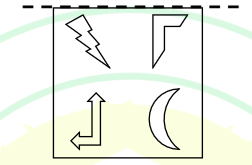
\includegraphics[width=0.5\columnwidth]{figs/01.jpg}
    \caption{}
    \label{fig:Img01}
    \end{figure}
    \begin{multicols}{2}
    \begin{enumerate}
        \item \begin{figure}[H]
    \centering
    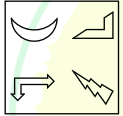
\includegraphics[width=0.5\columnwidth]{figs/02.jpg}
    \caption{}
    \label{fig:Img02}
    \end{figure}
        \item \begin{figure}[H]
    \centering
    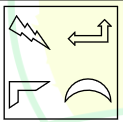
\includegraphics[width=0.5\columnwidth]{figs/03.jpg}
    \caption{}
    \label{fig:Img03}
    \end{figure}
        \item \begin{figure}[H]
    \centering
    
\includegraphics[width=0.5\columnwidth]{figs/04.jpg}
    \caption{}
    \label{fig:Img04}
    \end{figure}
        \item \begin{figure}[H]
    \centering
    
\includegraphics[width=0.5\columnwidth]{figs/05.jpg}
    \caption{}
    \label{fig:Img05}
    \end{figure}
    \end{enumerate}
    \end{multicols}
    \hfill (GATE-AR 2025)

    \item Which one of the following options has the correct sequence of objects arranged in the increasing number of mirror lines (lines of symmetry)?
    \begin{enumerate}
        \item Circle; Square; Equilateral triangle; Isosceles triangle
        \item Isosceles triangle; Equilateral triangle; Square; Circle
        \item Equilateral triangle; Isosceles triangle; Square; Circle
        \item Isosceles triangle; Square; Equilateral triangle; Circle
    \end{enumerate}
    \hfill (GATE-AR 2025)

    \item A final year student appears for placement interview in two companies, S and T. Based on her interview performance, she estimates the probability of receiving job offers from companies S and T to be 0.8 and 0.6, respectively. Let $p$ be the probability that she receives job offers from both the companies. Select the most appropriate option.
    \begin{multicols}{4}
    \begin{enumerate}
        \item $0 \leq p \leq 0.2$
        \item $0.4 \leq p \leq 0.6$
        \item $0.2 \leq p \leq 0.4$
        \item $0.6 \leq p \leq 1.0$
    \end{enumerate}
    \end{multicols}
    \hfill (GATE-AR 2025)

\section*{PART A: Common FOR ALL CANDIDATES}

    \item As per the United Nations Development Report, 1990, which of the following is NOT a key indicator of Human Development Index (HDI)?
    \begin{multicols}{2}
    \begin{enumerate}
        \item Life Expectancy at Birth
        \item Expected Years of Schooling
        \item Per capita Gross National Income (GNI)
        \item Mortality Rate
    \end{enumerate}
    \end{multicols}
    \hfill (GATE-AR 2025)

    \item As per the URDPFI Guidelines, 2015, the suggested population served by a single unit of neighbourhood park for plain areas is \rule{2cm}{0.4pt}.
    \begin{multicols}{4}
    \begin{enumerate}
        \item 5000
        \item 15000
        \item 35000
        \item 50000
    \end{enumerate}
    \end{multicols}
    \hfill (GATE-AR 2025)

    \item As per the National Building Code of India, 2016, the minimum clear opening width of a doorway to allow single wheelchair access, is \rule{2cm}{0.4pt} mm.
    \begin{multicols}{4}
    \begin{enumerate}
        \item 600
        \item 900
        \item 1200
        \item 1500
    \end{enumerate}
    \end{multicols}
    \hfill (GATE-AR 2025)

    \item In landscaping, Miyawaki technique is used for \rule{2cm}{0.4pt}.
    \begin{enumerate}
        \item creating waterbodies to stop rapid urbanization
        \item pruning shrubs in urban plantation
        \item creating dense forests with native plants
        \item identifying sites for urban vertical gardens
    \end{enumerate}
    \hfill (GATE-AR 2025)

    \item In Burgess's Concentric Zone model, 1920, \rule{2cm}{0.4pt} is characterized by mixed residential and commercial establishments.
    \begin{enumerate}
        \item Zone of better housing
        \item Zone of independent working class
        \item Zone of transition
        \item Zone of high-class homes on outskirts of outer suburbs
    \end{enumerate}
    \hfill (GATE-AR 2025)

    \item Identify the correct relationship with respect to water quality from the following options.
    \begin{enumerate}
        \item Total solids = Suspended solids + Dissolved solids + Colloidal solids
        \item Total gases = Biological Oxygen Demand + Chemical Oxygen Demand + Dissolved Oxygen
        \item Total solids = Suspended Solids + Dissolved solids
        \item Total gases = Biological Oxygen Demand + Chemical Oxygen Demand
    \end{enumerate}
    \hfill (GATE-AR 2025)

    \item As per the Solid Waste Management Rules, 2016, co-processing is the use of \rule{2cm}{0.4pt} and \rule{2cm}{0.4pt} solid waste having calorific value exceeding 1500 kcal/kg as raw material or as a source of energy, or both.
    \begin{enumerate}
        \item Non-biodegradable, Non-recyclable
        \item Biodegradable, Recyclable
        \item Non-biodegradable, Recyclable
        \item Biodegradable, Non-recyclable
    \end{enumerate}
    \hfill (GATE-AR 2025)

    \item For composting, the optimum Carbon to Nitrogen (C:N) ratio is closest to \rule{2cm}{0.4pt}.
    \begin{multicols}{4}
    \begin{enumerate}
        \item 5:1
        \item 30:1
        \item 70:1
        \item 1:1
    \end{enumerate}
    \end{multicols}
    \hfill (GATE-AR 2025)

    \item Read the following statements and select the correct option.\\    
    P: Strong axial layout, symmetry, proportion and infinite perspective of the 17th Century French Gardens reflects the wealth, power and rigid social structure of France.\\    
    Q: Italian gardens of early renaissance period were designed as intellectual retreats where scholars and artists could work and debate.
    \begin{multicols}{2}
    \begin{enumerate}
        \item P is true but Q is false
        \item P is false but Q is true
        \item Both P and Q are true
        \item Both P and Q are false
    \end{enumerate}
    \end{multicols}
    \hfill (GATE-AR 2025)

    \item The concept of \rule{2cm}{0.4pt} is primarily used to describe an urban area with plenty of green spaces and waterbodies to retain and/or detain rain water.
    \begin{multicols}{4}
    \begin{enumerate}
        \item Sponge City
        \item Aerocity
        \item 15-minute City
        \item Compact City
    \end{enumerate}
    \end{multicols}
    \hfill (GATE-AR 2025)

    \item Identify the correct sequence of drawings prepared by architects at various stages of building design and construction.
    \begin{enumerate}
        \item Working drawing; Statutory approval drawing; Conceptual design drawing; Completion drawing
        \item Statutory approval drawing; Conceptual design drawing; Completion drawing; Working drawing
        \item Conceptual design drawing; Statutory approval drawing; Working drawing; Completion drawing
        \item Conceptual design drawing; Working drawing; Completion drawing; Statutory approval drawing
    \end{enumerate}
    \hfill (GATE-AR 2025)

    \item As per the National Building Code of India, 2016, choose the correct option where materials are arranged in the increasing order of their embodied energy.
    \begin{enumerate}
        \item Medium Density Fibreboard < Aluminium < Float Glass < Fly-ash Bricks
        \item Fly-ash Bricks < Medium Density Fibreboard < Float Glass < Aluminium
        \item Medium Density Fibreboard < Fly-ash Bricks < Float Glass < Aluminium
        \item Fly-ash Bricks < Aluminium < Medium Density Fibreboard < Float Glass
    \end{enumerate}
    \hfill (GATE-AR 2025)

    \item Which one of the following Universal Design principles aims to "minimise hazards and the adverse consequences of accidental or unintended actions"?
    \begin{multicols}{2}
    \begin{enumerate}
        \item Flexibility in use
        \item Tolerance for error
        \item Perceptible information
        \item Simple and intuitive use
    \end{enumerate}
    \end{multicols}
    \hfill (GATE-AR 2025)

    \item Which one of the following buildings features an Onion dome?
    \begin{multicols}{2}
    \begin{enumerate}
        \item Matrimandir, Auroville
        \item Rashtrapati Bhavan, New Delhi
        \item Taj Mahal, Agra
        \item Victoria Memorial, Kolkata
    \end{enumerate}
    \end{multicols}
    \hfill (GATE-AR 2025)

    \item As per the UN's Sustainable Development Goals (SDGs), urban health is dealt with in SDG 3 and SDG 6 that are \rule{2cm}{0.4pt} and \rule{2cm}{0.4pt}, respectively.
    \begin{enumerate}
        \item Good health and well-being; Clean water and sanitation
        \item Reduced inequalities; High nutrition
        \item Reduced inequalities; Sustainable cities and communities
        \item Good health and well-being; High nutrition
    \end{enumerate}
    \hfill (GATE-AR 2025)

    \item The 4th and 5th dimension of Building Information Modelling (BIM) are \rule{2cm}{0.4pt} and \rule{2cm}{0.4pt}, respectively.
    \begin{enumerate}
        \item Facility management; Sustainability
        \item Construction schedule; Construction costing
        \item Sustainability; Construction schedule
        \item Construction costing; Facility management
    \end{enumerate}
    \hfill (GATE-AR 2025)

    \item Which of the following is/are likely to be caused by an earthquake?
    \begin{multicols}{4}
    \begin{enumerate}
        \item Liquefaction
        \item Heatwave
        \item Tsunami
        \item Tornado
    \end{enumerate}
    \end{multicols}
    \hfill (GATE-AR 2025)

    \item Which of the following cities predominantly has/have a grid iron street pattern?
    \begin{multicols}{4}
    \begin{enumerate}
        \item Cairo
        \item Chandigarh
        \item Philadelphia
        \item Venice
    \end{enumerate}
    \end{multicols}
    \hfill (GATE-AR 2025)

    \item Match the following items of work in \textbf{Group-I} with their corresponding units of measurement in \textbf{Group-II}. \\
    \begin{tabular}{ l l }
    \textbf{Group-I} & \textbf{Group-II} \\
    (P) Honeycomb Brickwork & (1) Running Meter \\
    (Q) Steel Reinforcement & (2) Cubic Meter \\
    (R) Brick on Edge & (3) Square Meter \\
    (S) Earthwork in Excavation & (4) Kilogram \\
    & (5) Number \\
    \end{tabular}
    \begin{multicols}{2}
    \begin{enumerate}
        \item P-1, Q-4, R-3, S-2
        \item P-3, Q-1, R-4, S-5
        \item P-5, Q-2, R-1, S-4
        \item P-3, Q-4, R-1, S-2
    \end{enumerate}
    \end{multicols}
    \hfill (GATE-AR 2025)

    \item Match the types of water carriage system in \textbf{Group-I} with their corresponding functions in \textbf{Group-II}. \\
    \begin{tabular}{ l l }
    \textbf{Group-I} & \textbf{Group-II} \\
    (P) Combined system & (1) Rain water from roof is allowed to \\
    & enter the sewer carrying sewage and \\
    & the remaining storm water flows \\
    & separately \\
    (Q) Vacuum sewer system & (2) Rain water from roof and sewage \\
    & from buildings are taken along with \\
    & storm water \\
    (R) Partially separate & (3) A pump is used to pump waste from \\
    system & the residences to the low pressure \\
    & sewer line \\
    (S) Pressurized sewer & (4) The sewer is under negative \\
    system & pressure and it pulls sewage and air \\
    & from different sources \\
    & (5) Sewage from buildings is taken in \\
    & one set of sewers and storm water in \\
    & another network \\
    \end{tabular}
    \begin{multicols}{2}
    \begin{enumerate}
        \item P-2, Q-4, R-1, S-3
        \item P-2, Q-3, R-5, S-4
        \item P-1, Q-4, R-5, S-3
        \item P-1, Q-3, R-1, S-4
    \end{enumerate}
    \end{multicols}
    \hfill (GATE-AR 2025)

    \item Match the following UNESCO World heritage sites in \textbf{Group-I} with their relevant historic significance in \textbf{Group-II}. \\
    \begin{tabular}{ l l }
    \textbf{Group-I} & \textbf{Group-II} \\
    (P) Walled City of Jaipur & (1) A city from the Mughal era, \\
    & planned as a whole with \\
    & architectural ensembles constructed \\
    & at the end of 16\textsuperscript{th} Century \\
    (Q) Fatehpur Sikri & (2) Timber based architecture of \\
    & historic city, having exceptional \\
    & significance from 15\textsuperscript{th} Century \\
    & Sultanate period \\
    (R) Group of Monuments at & (3) Conceived in a single phase in the \\
    Hampi & 18\textsuperscript{th} Century with a gird-iron pattern \\
    & inspired from prastara plan of \\
    & vāstushāstra \\
    (S) Dholavira, Harappan & (4) Comprises mainly the remnants of \\
    city & the capital city of Vijayanagara \\
    & Empire \\
    & (5) Proto-historic bronze age urban \\
    & settlement \\
    \end{tabular}
    \begin{multicols}{2}
    \begin{enumerate}
        \item P-1, Q-2, R-4, S-5
        \item P-5, Q-1, R-3, S-4
        \item P-3, Q-1, R-4, S-5
        \item P-3, Q-5, R-2, S-4
    \end{enumerate}
    \end{multicols}
    \hfill (GATE-AR 2025)

    \item Match the following principles of design in \textbf{Group–I} to their corresponding descriptions in \textbf{Group–II}. \\
\begin{tabular}{ l l }
\textbf{Group–I} & \textbf{Group–II} \\
(P) Datum & (1) The use of recurring patterns to organize a \\
& series of like forms or spaces \\
(Q) Symmetry & (2) The balanced distribution of equivalent \\
& forms and spaces about a common line or \\
& point \\
(R) Hierarchy & (3) A line established by two points in space, \\
& about which forms and spaces can be \\
& arranged in a symmetrical or balanced \\
& manner \\
(S) Rhythm & (4) A line, plane or volume that by its \\
& continuity and regularity helps to organize \\
& a pattern of forms and spaces \\
& (5) The significance of a form or space based \\
& in the size, shape or placement relative to \\
& other forms of the organization \\
\end{tabular}
\begin{multicols}{2}
\begin{enumerate}
    \item P-3, Q-2, R-5, S-1
    \item P-4, Q-1, R-3, S-5
    \item P-4, Q-2, R-5, S-1
    \item P-3, Q-4, R-2, S-5
\end{enumerate}
\end{multicols}
\hfill (GATE-AR 2025)

\item Match the following Books in \textbf{Group–I} with their corresponding Authors in \textbf{Group–II}. \\
\begin{tabular}{ l l }
\textbf{Group–I} & \textbf{Group–II} \\
(P) Cities for People & (1) Francis D. K. Ching \\
(Q) Architecture: Form, Space, & (2) Jan Gehl \\
and Order & \\
(R) The Death and Life of Great & (3) Kevin Lynch \\
American Cities & \\
(S) The Image of the City & (4) Jane Jacobs \\
& (5) F. L. Wright \\
\end{tabular}
\begin{multicols}{2}
\begin{enumerate}
    \item P-5, Q-2, R-4, S-3
    \item P-2, Q-1, R-4, S-3
    \item P-3, Q-4, R-5, S-1
    \item P-2, Q-1, R-3, S-4
\end{enumerate}
\end{multicols}
\hfill (GATE-AR 2025)

\item In order to achieve the static equilibrium of the see-saw about the fulcrum \textbf{P}, shown in the \figref{fig:Img06}, the weight of the Box \textbf{B} should be \rule{2cm}{0.4pt} kg, if weight of Box A is 50 kg.
\begin{figure}[h!]
\centering
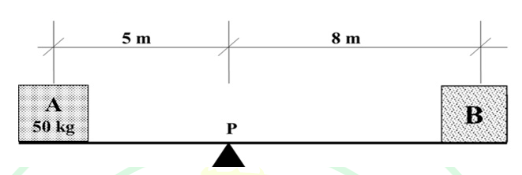
\includegraphics[width=0.5\columnwidth]{figs/06.jpg}
\caption{}
\label{fig:Img06}
\end{figure}
\begin{multicols}{4}
\begin{enumerate}
    \item 50
    \item 31.25
    \item 80
    \item 61.25
\end{enumerate}
\end{multicols}
\hfill (GATE-AR 2025)

\item Which of the following is/are supply side intervention(s) to improve housing affordability?
\begin{enumerate}
    \item Increase in availability of urban land for housing
    \item Increase in Institutional Housing Finance
    \item Reduction in Floor Area Ratio
    \item Increase in Stamp Duty
\end{enumerate}
\hfill (GATE-AR 2025)

\item Which of the following method(s) is/are used for desalination of water?
\begin{multicols}{2}
\begin{enumerate}
    \item Reverse Osmosis
    \item Activated Sludge Process
    \item Incineration
    \item Distillation
\end{enumerate}
\end{multicols}
\hfill (GATE-AR 2025)

\item Identify the set(s) of complimentary colours based on RGB Model.
\begin{enumerate}
    \item Yellow and Purple
    \item Yellow and Orange
    \item Blue and Orange
    \item Blue and Purple
\end{enumerate}
\hfill (GATE-AR 2025)

    \item A city has a population of 1,75,000. Using the Kuichling's formula the estimated fire demand for the city is \rule{2cm}{0.4pt} litres/min. (rounded off to two decimal places) \\
    \hfill (GATE-AR 2025)

    \item A rectangular plot has the dimensions of 20 m $\times$ 15 m. A building on the plot fully utilizes both Floor Area Ratio (FAR) of 3.0 and ground coverage of 50\%. Considering all floors having equal area, the maximum number of floors that can be built on the plot is \rule{2cm}{0.4pt}. (answer in integer) \\
    \hfill (GATE-AR 2025)

    \item A real estate project on a 12 hectare site contains 6 buildings, each with ground coverage of 3 percent of the site area. The landscaped area is 40 percent of the site and rest of the area are roads. Assume coefficient of runoff for landscaped area and road area to be 0.15 and 0.6 respectively. Ignore the rainwater from the roof of the buildings and additional water from outside areas. Considering average rainfall intensity of 70 mm per hour, the estimated peak surface runoff rate from the site is \rule{2cm}{0.4pt} m$^3$/s. (rounded off to two decimal places) \\
    \hfill (GATE-AR 2025)
    
    \item In a regular semi-circular arch of 2 m clear span, the thickness of the arch is 30 cm and the breadth of the wall is 40 cm. The total quantity of brickwork in the arch is \rule{2cm}{0.4pt} m$^3$. (rounded off to two decimal places) \\
    \begin{figure}[h!]
    \centering
    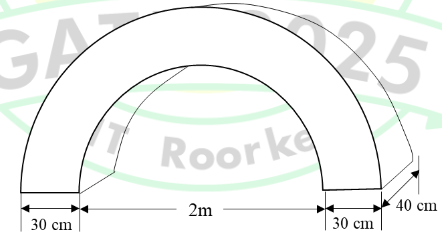
\includegraphics[width=0.5\columnwidth]{figs/07.jpg}
    \caption{}
    \label{fig:Img07}
    \end{figure}
    \hfill (GATE-AR 2025)

    \item A roof area of 6000 m$^2$ of a building is drafted on a drawing sheet as 240 cm$^2$. The scale used in the drawing sheet is 1:\rule{2cm}{0.4pt}. (rounded off to the nearest integer) \\
\hfill (GATE-AR 2025)

\item A housing property of INR 50 lakh is on sale either through a Full Down Payment (FDP) scheme with an 8\% rebate OR a Deferred Payment Plan (DPP) as shown in the table. A customer after converting all the future payments in DPP using 10\% annual discount rate, found the DPP scheme to be financially gainful. The customer would be able to save in INR \rule{2cm}{0.4pt} lakh, if DPP is chosen over FDP. (rounded off to two decimal places) \\
\begin{tabular}{ | l | l | }
\hline
\multicolumn{2}{|c|}{Deferred Payment Plan (DPP)} \\
\hline
At the time of booking & INR 10 lakh \\
\hline
After one year & INR 15 lakh \\
\hline
After two year & INR 15 lakh \\
\hline
After three year & INR 10 lakh \\
\hline
\end{tabular} \\
\hfill (GATE-AR 2025)

\item The population of a city in the year 2001, 2011, 2021 were recorded as 52,000, 76,000 and 1,20,000 respectively. Calculating the average growth rate using geometric mean, the estimated population of the city for 2031 using geometric increase method is \rule{2cm}{0.4pt}. (rounded off to the nearest integer) \\
\hfill (GATE-AR 2025)

\item A room having dimension of 12 m $\times$ 8 m and height 4 m, stores a certain combustible material of volume 80 m$^3$. The density and calorific value of the combustible material are 3.0 kg/m$^3$ and 4000 kcal/kg, respectively. The fire load of the room is \rule{2cm}{0.4pt} kcal/m$^2$. (rounded off to the nearest integer) \\
\hfill (GATE-AR 2025)

\item A construction project consists of four activities. The duration, relationship and cost parameters are given in the table. The indirect cost of the project is INR 5000/- per week. If the project has to be completed by 12 weeks, the total project cost will be, INR\rule{2cm}{0.4pt}. (Answer in integer) \\
\begin{tabular}{ | l | c | c | c | c | c | }
\hline
Activity & Immediate & Normal & Crash & Normal & Crash Cost \\
& Predecessor & Duration & Duration & Cost (INR) & (INR) \\
& Activity & (Weeks) & (Weeks) & & \\
\hline
P & Nil & 8 & 5 & 20,000 & 26,000 \\
\hline
Q & Nil & 5 & 2 & 30,000 & 33,000 \\
\hline
R & P & 6 & 4 & 40,000 & 52,000 \\
\hline
S & Q & 4 & 3 & 10,000 & 13,000 \\
\hline
\end{tabular} \\
\hfill (GATE-AR 2025)

\item A 24 cm line AB is vertically standing on a horizontal plane. The station point is located 18 cm above ground and 15 cm in front of the line AB. The picture plane is located in between the line AB and station point perpendicular to the sight line. The distance between the picture plane and the station point is 9 cm. The height of the perspective view of the line AB is \rule{2cm}{0.4pt} cm. (rounded off to one decimal place) \\
\hfill (GATE-AR 2025)

\item The view from ground to sky of a location is projected on a plane as shown in the figure. The hatched and the solid black portion of the diagram represent the sky and the obstructions, respectively. The radius of the whole circle shown in the figure is 3 units and other dimensions are provided in \figref{fig:Img08}. The Sky View Factor (SVF) of this location is \rule{2cm}{0.4pt}. (rounded off to two decimal places) \\
\begin{figure}[h!]
\centering
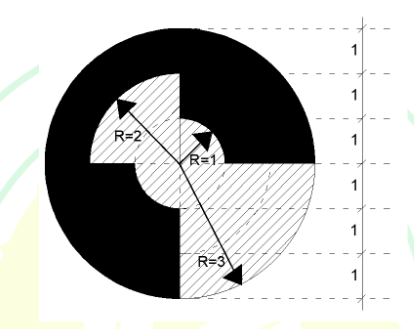
\includegraphics[width=0.4\columnwidth]{figs/08.jpg}
\caption{}
\label{fig:Img08}
\end{figure}
\hfill (GATE-AR 2025)

\newpage

\item A city aims to introduce Metro rail as a sustainable public transport, with a projected daily ridership of 3,67,200 which is expected to shift 18\% of the daily trips from other existing modes. The existing modal share (in percentage) is shown in \figref{fig:Img09}. If half of the above modal shift is expected to replace trips by Motorised Two-wheeler and Motorised Four-wheeler in 2:1 ratio, the trips only by Motorised Two-wheeler, post modal shift to Metro is \rule{2cm}{0.4pt}. (answer in integer) \\
\begin{figure}[h!]
\centering
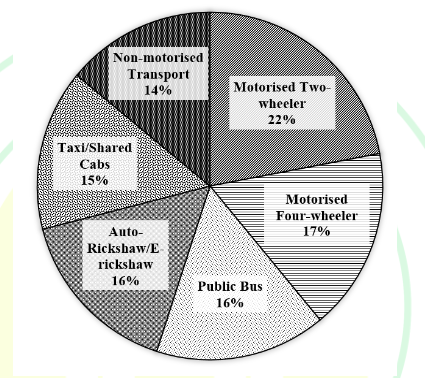
\includegraphics[width=0.5\columnwidth]{figs/09.jpg}
\caption{}
\label{fig:Img09}
\end{figure}
\hfill (GATE-AR 2025)

\section*{PART B1: FOR Architecture CANDIDATES ONLY}

    \item With reference to Squinch adopted in dome construction, choose the correct option related to statements P and Q. \\    
    P: Squinch is a structural element used to support the base of a circular or octagonal dome that surmounts a square hall. \\    
    Q: Squinch is a double layered dome comprising of an inner and an outer layer of masonry.
    \begin{multicols}{2}
    \begin{enumerate}
        \item Both P and Q are true
        \item P is true but Q is false
        \item P is false but Q is true
        \item Both P and Q are false
    \end{enumerate}
    \end{multicols}
    \hfill (GATE-AR 2025)

    \item In Heating Ventilation and Air Conditioning (HVAC) systems, HVAC dampers are essentially \rule{2cm}{0.4pt}.
    \begin{enumerate}
        \item valves that regulate the airflow as per the air-conditioned zone requirements
        \item valves that regulate the refrigerant flow as per the air-conditioned zone requirements
        \item desiccants which are used to absorb the moisture and dehumidify the air-conditioned zone
        \item metal-based sheets to absorb heat and to cool the air-conditioned zone
    \end{enumerate}
    \hfill (GATE-AR 2025)

    \item \rule{2cm}{0.4pt} increases the spreading quality of paints and helps to achieve desired consistency.
    \begin{multicols}{4}
    \begin{enumerate}
        \item Base
        \item Vehicle
        \item Paint Drier
        \item Solvent
    \end{enumerate}
    \end{multicols}
    \hfill (GATE-AR 2025)

\newpage

    \item The graph in \figref{fig:Img10} shows the typical test result of a property of a building material. Identify the test and the variables represented on the X-axis and Y-axis from the given options.
\begin{figure}[h!]
\centering
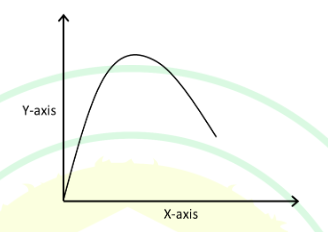
\includegraphics[width=0.5\columnwidth]{figs/10.jpg}
\caption{}
\label{fig:Img10}
\end{figure}
\begin{enumerate}
    \item Workability test of concrete; X-Axis: water-cement ratio; Y-Axis: amount of slump
    \item Cube test of concrete; X-Axis: water-cement ratio; Y-Axis: 28-days compressive strength
    \item Ultrasonic pulse velocity test; X-Axis: pulse velocity; Y-Axis: compressive strength
    \item Bulking test of sand; X-Axis: moisture percentage; Y-Axis: percentage increase in volume
\end{enumerate}
\hfill (GATE-AR 2025)

\item A typical Classical Greek temple with Doric order columns is illustrated in \figref{fig:Img11}. Identify the correct terms corresponding to P, Q and R marked in \figref{fig:Img11}.
\begin{figure}[h!]
\centering
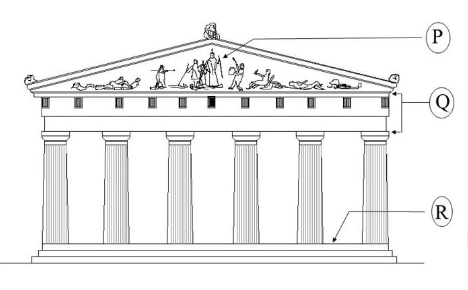
\includegraphics[width=0.5\columnwidth]{figs/11.jpg}
\caption{}
\label{fig:Img11}
\end{figure}
\begin{enumerate}
    \item P-Cella; Q-Entablature; R-Tympanum
    \item P-Tympanum; Q-Entablature; R-Stylobate
    \item P-Tympanum; Q-Acroterium; R-Stylobate
    \item P-Cella; Q-Stylobate; R-Acroterium
\end{enumerate}
\hfill (GATE-AR 2025)

\item Which of the following is/are example(s) of Concrete Cased Pile?
\begin{multicols}{2}
\begin{enumerate}
    \item Raymond Pile
    \item Swage Pile
    \item Vibro Pile
    \item Simplex Pile
\end{enumerate}
\end{multicols}
\hfill (GATE-AR 2025)

\item For a given location, the Sun's position is at 40$\degree$ Altitude angle and 130$\degree$ N Azimuth angle. The Zenith Angle of the Sun (in degree) at that given location is \rule{2cm}{0.4pt}. \\
\hfill (GATE-AR 2025)

\item Match the items in \textbf{Group–I} with the corresponding items in \textbf{Group–II}. \\
\begin{tabular}{ l l }
\textbf{Group–I} & \textbf{Group–II} \\
(P) Garmet & (1) Lock \\
(Q) Aldrop & (2) Screw \\
(R) Mortise & (3) Bolt \\
(S) Gusset & (4) Hinge \\
& (5) Plate \\
\end{tabular}
\begin{multicols}{2}
\begin{enumerate}
    \item P–4, Q–3, R–1, S–5
    \item P-5, Q-3, R-4, S–2
    \item P–4, Q–1, R–3, S–5
    \item P–3, Q–2, R–1, S–4
\end{enumerate}
\end{multicols}
\hfill (GATE-AR 2025)

\item Match the statements in \textbf{Group–I} with the corresponding names of architects in \textbf{Group–II}. \\
\begin{tabular}{ l l }
\textbf{Group–I} & \textbf{Group–II} \\
(P) Form Follows Function & (1) Ludwig Mies van der Rohe \\
(Q) Less is More & (2) Louis H. Sullivan \\
(R) Architecture should speak of its & (3) Antoni Gaudi \\
time and place, but yearn for & \\
timelessness & \\
(S) There are no straight lines or & (4) Frank O. Gehry \\
sharp corners in nature & \\
& (5) Adolf Loos \\
\end{tabular}
\begin{multicols}{2}
\begin{enumerate}
    \item P–1, Q–2, R–4, S–5
    \item P–2, Q–3, R–1, S–4
    \item P–2, Q–1, R–4, S–3
    \item P–5, Q–1, R–2, S–3
\end{enumerate}
\end{multicols}
\hfill (GATE-AR 2025)

\item Match the items in \textbf{Group–I} with the corresponding statements in \textbf{Group–II}. \\
\begin{tabular}{ l l }
\textbf{Group–I} & \textbf{Group–II} \\
(P) Suction lift & (1) Difference between point of discharge \\
& and the pump \\
(Q) Discharge lift & (2) Filling pump casing with air to remove \\
& trapped air inside \\
(R) Rotary pump & (3) Difference between low water level and \\
& pump \\
(S) Priming of pump & (4) Water is carried upwards around the side \\
& of the casing and pushed through \\
& discharge pipe \\
& (5) Work done by a pump in raising the \\
& water \\
\end{tabular}
\begin{multicols}{2}
\begin{enumerate}
    \item P–3, Q–1, R–4, S–2
    \item P–4, Q–5, R–3, S–1
    \item P–3, Q–1, R–5, S–4
    \item P–1, Q–5, R–4, S–2
\end{enumerate}
\end{multicols}
\hfill (GATE-AR 2025)

\item Match the following Indian Temples in \textbf{Group–I} with their relevant descriptions in \textbf{Group–II}. \\
\begin{tabular}{ l l }
\textbf{Group–I} & \textbf{Group–II} \\
(P) Kailasa Temple, Ellora & (1) Temple from Chandella culture \\
(Q) Shore Temple, & (2) Temple from late Gupta period \\
Mamallapuram & entirely built in brick \\
(R) Mahabodhi Temple, & (3) Pallava temple constructed of dressed \\
Bodh Gaya & stone \\
(S) Brihadisvara Temple, & (4) Brahmanical rock-cut architecture, \\
Thanjavur & constructed by excavating out of the \\
& hill site \\
& (5) One of the largest Chola temples \\
\end{tabular}
\begin{multicols}{2}
\begin{enumerate}
    \item P–1, Q–3, R–2, S–4
    \item P–4, Q–2, R–5, S–3
    \item P–3, Q–4, R–1, S–5
    \item P–4, Q–3, R–2, S–5
\end{enumerate}
\end{multicols}
\hfill (GATE-AR 2025)

\item Which of the following tall building(s) is/are having bundled-tube structural system?
\begin{enumerate}
    \item Sears Tower, Chicago
    \item The 42, Kolkata
    \item O-16 Building, Dubai
    \item Bank of China, Hong Kong
\end{enumerate}
\hfill (GATE-AR 2025)

\item A simply supported beam is under a uniformly distributed load (UDL) along the full span. The mid-span deflection is measured as 24 mm. If the length and depth of the beam is doubled while keeping other parameters unchanged, the mid-span deflection is \rule{2cm}{0.4pt} mm. (answer in integer) \\
\hfill (GATE-AR 2025)

\item A rectangular RCC beam section of 250 mm width and 400 mm effective depth is under a factored Shear Force of 120 kN. The design shear strength ($\tau_c$) of concrete is 0.35 N/mm$^2$. Two-legged, 8 mm diameter stirrups are used for the shear reinforcement. Assuming the Yield Stress of Steel, $f_y = 415$ N/mm$^2$, the design spacing (c/c) of the stirrups is \rule{2cm}{0.4pt} mm. (rounded off to the nearest integer) \\
\hfill (GATE-AR 2025)

\item A source of light is located at point C. Point A is 1.75 m vertically below point C. Point B is situated horizontally 1.0 m right of point A. If the illumination level at point A due to the light source at point C is 300 Lux, then the illumination level at point B is \rule{2cm}{0.4pt} Lux. (rounded off to the nearest integer) \\
\hfill (GATE-AR 2025)

\item There are 16 similar machines located radially and equally distanced from a fixed sound receiver. While operating, each machine records 60 dB sound level at the receiver. Assuming 70 dB to be the highest sound level allowed as per the industrial sound pollution norms, the total number of machines allowed to operate simultaneously without violating the norms is \rule{2cm}{0.4pt}. (rounded off to the nearest integer) \\
\hfill (GATE-AR 2025)

\section*{PART B2: FOR Planning CANDIDATES ONLY}

    \item Affordable Housing in Partnership (AHP) is one of the verticals of Pradhan Mantri Awas Yojana (PMAY) of Government of India. In AHP, the partnership was envisaged between \rule{2cm}{0.4pt}.
    \begin{enumerate}
        \item States/UTs/ULBs/Parastatals and Academic Institutions
        \item States/UTs/ULBs/Parastatals and Private Developers
        \item Non-Government Organisation (NGO) and Private Developers
        \item Non-Government Organisation (NGO) and Academic Institutions
    \end{enumerate}
    \hfill (GATE-AR 2025)

    \item Which are the two wavelength bands of light spectrum used to calculate the Normalised Difference Vegetation Index (NDVI) in remote sensing?
    \begin{multicols}{2}
    \begin{enumerate}
        \item Green and Blue
        \item Green and Near Infrared
        \item Near Infrared and Red
        \item Red and Green
    \end{enumerate}
    \end{multicols}
    \hfill (GATE-AR 2025)

    \item \rule{2cm}{0.4pt} refers to the benefits when industries/firms cluster together resulting in reduced production cost, improved availability of skilled labor, and increased flow of information and knowledge sharing.
    \begin{multicols}{2}
    \begin{enumerate}
        \item Industrial ecology
        \item Agglomeration of economies
        \item Behavioural economics
        \item Industrial engineering
    \end{enumerate}
    \end{multicols}
    \hfill (GATE-AR 2025)
    
    \item As per the Right to Fair Compensation and Transparency in Land Acquisition, Rehabilitation and Resettlement Act, 2013, the \rule{2cm}{0.4pt} determines the \rule{2cm}{0.4pt} for compensation for land acquisition.
\begin{multicols}{2}
\begin{enumerate}
    \item Collector; market value
    \item Planning Officer; market value
    \item Collector; circle rate
    \item Planning Officer; circle rate
\end{enumerate}
\end{multicols}
\hfill (GATE-AR 2025)

\item Total Station is an equipment used for \rule{2cm}{0.4pt}.
\begin{enumerate}
    \item measurement of rainfall intensity
    \item noise level measurement
    \item air quality measurement
    \item determination of coordinates of unknown points relative to a known coordinate
\end{enumerate}
\hfill (GATE-AR 2025)

\item Select the correct statement(s) with regard to Traffic Analysis Zones (TAZs).
\begin{enumerate}
    \item TAZs are not determined based on physical barriers like rivers, mountains and forest.
    \item Demographic characteristics of a TAZ will change with new residents moving into the TAZ.
    \item 'Cordon line' helps in defining the study area within which TAZs are located.
    \item TAZs cannot include multiple wards.
\end{enumerate}
\hfill (GATE-AR 2025)

\item As per the Census of India, 2011, choose the correct statement(s), regarding the definition of a Census Town.
\begin{enumerate}
    \item The minimum population size is 5000.
    \item The population density of at least 400 persons per square kilometer.
    \item 55 percent of the male working population are not engaged in agriculture.
    \item The population density of at least 250 persons per square kilometer.
\end{enumerate}
\hfill (GATE-AR 2025)

\item Match the following Planning Strategies in \textbf{Group–I} to their corresponding descriptions in \textbf{Group–II}. \\
\begin{tabular}{ l l }
\textbf{Group–I} & \textbf{Group–II} \\
(P) Urban Sprawl & (1) Redeveloping previously utilized \\
& land, often resulting in a change in \\
& land-use and land cover \\
(Q) Smart Growth & (2) Development on previously \\
& undeveloped land \\
(R) Greenfield Development & (3) Concentrating development in \\
& compact, walkable urban centres to \\
& improve health and natural \\
& environment \\
(S) Brownfield & (4) Expansion of urban areas into rural \\
Development & areas, typically characterized by low- \\
& density development \\
& (5) Allocating specific areas for industrial \\
& activities to minimize environmental \\
& impacts and segregate them from \\
& residential areas \\
\end{tabular}
\begin{multicols}{2}
\begin{enumerate}
    \item P–4, Q–2, R–5, S–1
    \item P–1, Q–2, R–3, S–4
    \item P–4, Q–3, R–2, S–1
    \item P–1, Q–3, R–2, S–5
\end{enumerate}
\end{multicols}
\hfill (GATE-AR 2025)

\item Match the following sub categories of urban land use in \textbf{Group–I} with their corresponding broad land use categories in \textbf{Group–II} as per URDPFI Guidelines, 2015. \\
\begin{tabular}{ l l }
\textbf{Group–I} & \textbf{Group–II} \\
(P) Sports complex & (1) Protective and undevelopable use zone \\
(Q) Water bodies & (2) Recreational \\
(R) Poultry and dairy & (3) Special area \\
farming & \\
(S) Police station & (4) Primary Activity \\
& (5) Public and Semi-Public \\
\end{tabular}
\begin{multicols}{2}
\begin{enumerate}
    \item P–2, Q–1, R–4, S–5
    \item P–3, Q–2, R–1, S–3
    \item P–4, Q–2, R–3, S–5
    \item P–2, Q–4, R–5, S–3
\end{enumerate}
\end{multicols}
\hfill (GATE-AR 2025)

\item Match the following Curves in \textbf{Group–I} with their corresponding uses in \textbf{Group–II}. \\
\begin{tabular}{ l l }
\textbf{Group–I} & \textbf{Group–II} \\
(P) Mass Curve & (1) A graphical representation of income or \\
& wealth inequality \\
(Q) Lorenz Curve & (2) A graphical representation of cumulative \\
& inflow (supply) and outflow(demand) over \\
& time \\
(R) Density Curve & (3) Shows the relationship between the price \\
& of a good or service and the quantity \\
& demanded within a specified time frame \\
(S) Horizontal Curve & (4) Provides a transition between tangent \\
& strips of roadway allowing a vehicle to \\
& negotiate a turn \\
& (5) An idealised representation of distribution \\
& in which the area under the curve is \\
& defined to be 1 \\
\end{tabular}
\begin{multicols}{2}
\begin{enumerate}
    \item P–2, Q–3, R–4, S–5
    \item P–3, Q-1, R–5, S–2
    \item P–1, Q–2, R–3, S–4
    \item P–2, Q–1, R–5, S–4
\end{enumerate}
\end{multicols}
\hfill (GATE-AR 2025)

\item Match the following types of migration in \textbf{Group–I} to their corresponding descriptions in \textbf{Group– II}. \\
\begin{tabular}{ l l }
\textbf{Group–I} & \textbf{Group–II} \\
(P) Involuntary migration & (1) When a migrant follows a path or series \\
& of stages towards a final destination \\
(Q) Step migration & (2) Repetitive movement of a migrant \\
& worker between home and destination \\
& areas \\
(R) Circular migration & (3) Forced displacement from their origin \\
& to destination areas \\
(S) Chain migration & (4) Immigrants from a particular area \\
& follow others from that area to a \\
& particular destination \\
& (5) Relocation or process of people \\
& leaving one country to reside in another \\
\end{tabular}
\begin{multicols}{2}
\begin{enumerate}
    \item P–2, Q–3, R–4, S–1
    \item P–3, Q–1, R–2, S–4
    \item P–3, Q–1, R–5, S–4
    \item P–1, Q–4, R–2, S–3
\end{enumerate}
\end{multicols}
\hfill (GATE-AR 2025)

\item Which of the following characteristics of a house or land is/are considered in hedonic price function?
\begin{enumerate}
    \item Quality of the view from the house
    \item Low crime rate in the surrounding area
    \item Number of bedrooms in the house
    \item Household size
\end{enumerate}
\hfill (GATE-AR 2025)

\item Which of the following is/are the characteristics of urban agglomeration as per the Census of India, 2011?
\begin{enumerate}
    \item A continuous urban spread constituting a town and its adjoining outgrowths
    \item Urban settlements combined with one rural settlement
    \item Two or more contiguous towns together with or without outgrowths
    \item Urban villages engulfed within a metropolitan area
\end{enumerate}
\hfill (GATE-AR 2025)

    \item The spot speeds (in km/h) of eight vehicles in a traffic stream are 42, 52, 56, \textbf{X}, 53, 62, 65, and 48. \textbf{X} is the spot speed of the fourth vehicle. The Time Mean Speed of the traffic stream is 56.25 km/h. After determining the value of \textbf{X}, the calculated Space Mean Speed of the traffic stream is \rule{2cm}{0.4pt} km/h. (rounded off to two decimal places) \\
    \hfill (GATE-AR 2025)
    
    \item An individual chooses a transport mode for a particular trip based on three attributes
i.e., cost of journey (X), In-vehicle travel time to reach destination (Y), and Out-of-
vehicle time taken to access mode at respective stops (Z). The values for these
attributes for three modes Rail, Bus and Para-transit are given in the table. If the
general utility (U) equation is $U = - 0.5 \times X – 0.3 \times Y – 0.4 \times Z$, using Logit model, the estimated probability of choosing Bus is \rule{2cm}{0.4pt}. (rounded off to
two decimal places) \\
    \begin{tabular}{ |l|c|c|c|}
    \hline
    Mode & X=Cost of & Y=In-Vehicle & Z=Out-of-Vehicle \\
    & journey (in INR) & travel time (in min) & travel time (in min) \\
    \hline
    Rail & 20 & 20 & 10 \\
    \hline
    Bus & 10 & 40 & 7.5 \\
    \hline
    Para-transit & 15 & 35 & 5 \\
    \hline
    \end{tabular}

    \item A four-arm uncontrolled un-signalized urban intersection of both way traffic is illustrated in \figref{fig:Img12}. Vehicles approaching the intersection from the directions A, B, C, and D can move to either left, right, or continue in straight direction. No U-turn is allowed. In the given situation, the maximum number of vehicular crossing conflict points for this intersection is \rule{2cm}{0.4pt}. (answer in integer) \\
    \begin{figure}[h!]
    \centering
    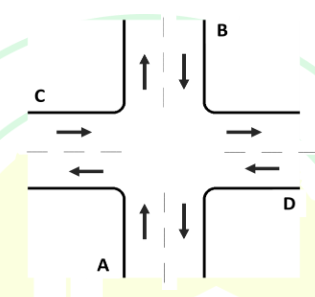
\includegraphics[width=0.3\columnwidth]{figs/12.jpg}
    \caption{}
    \label{fig:Img12}
    \end{figure}
    \hfill (GATE-AR 2025)

\end{enumerate}

\centering
\section*{END OF THE QUESTION PAPER}

\end{document}
